\documentclass[11pt]{scrartcl}
\usepackage[utf8]{inputenc}
\usepackage[sexy]{evanchen} 
\usepackage{graphicx}
\graphicspath{{8 Outsource K Math/Gambar/}}

\title{Kolinearitas dan Konkurensi}
\author{Azzam and Akeyla}
\date{Januari 2020}

\begin{document}

\maketitle

\section{Kolinearitas}
Tiga titik dikatakan kolinear/segaris jika ada sebuah garis yang melewati ketiga titik tersebut. 
\subsection{Menelaus}
\begin{theorem}
    [Teorema Menelaus] Misalkan $ABC$ adalah sebuah segitiga. Titik $D,E,F$ secara berturut-turut terletak di sisi $BC,CA,AB$ sedemikian hingga sebanyak ganjil ($1$ atau $3$) di antaranya terletak di perpanjangan sisi. Titik $D,E,F$ kolinear jika dan hanya jika
$$\dfrac{AF}{FB}\cdot \dfrac{BD}{DC} \cdot \dfrac{CE}{EA} = 1$$    
\end{theorem}

\begin{figure}[h]
    \centering
    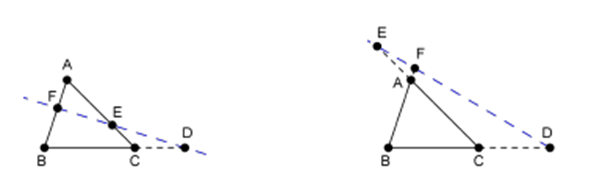
\includegraphics[width=0.8\linewidth]{menelaus.png}
\end{figure}

\subsection{Pengecekan dengan Sudut}
Secara manual, membuktikan tiga titik A,B,C kolinear bisa dengan salah satu dari ketiga cara berikut:
\begin{figure}[h]
    \centering
    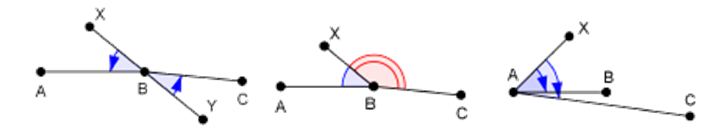
\includegraphics[width=0.8\linewidth]{kolinkonku.png}
\end{figure}
\begin{enumerate}
\item Tentukan sebuah garis yang memuat tiga titik: $X,B,Y$. Jika kita dapat membuktikan $\angle{XBA}= \angle{YBC}$, maka $A,B,C$ kolinear.
\item Tentukan sebuah titik $X$. Jika kita dapat membuktikan kalau $\angle{XBA}+ \angle{XBC}=180^{\circ}$, maka $A,B,C$ kolinear.
\item Tentukan sebuah titik $X$. Jika kita dapat membuktikan kalau $\angle{XAB}= \angle{XAC}$, maka $A,B,C$ kolinear.
\end{enumerate}

\section{Konkurensi}
Tiga garis dikatakan konkuren jika ketiga garis tersebut melewati sebuah titik yang sama di bidang. 
\subsection{Ceva}
\begin{theorem}
    [Teorema Ceva] Misalkan $ABC$ adalah sebuah segitiga. Titik $D,E,F$ secara berturut-turut terletak di sisi $BC,CA,AB$ sedemikian hingga sebanyak genap ($0$ atau $2$) di antaranya terletak di perpanjangan sisi. Garis $AD,BE,CF$ konkuren atau saling paralel jika dan hanya jika $$\dfrac{AF}{FB}\cdot \dfrac{BD}{DC} \cdot \dfrac{CE}{EA} = 1$$
\end{theorem}

\begin{figure}[h]
    \centering
    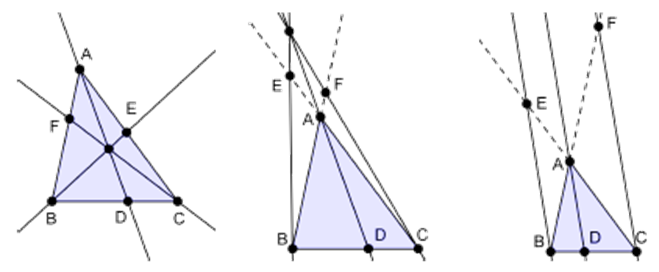
\includegraphics[width=0.8\linewidth]{ceva.png}
\end{figure}

Terdapat variasi teorema Ceva yang menggunakan trigonometri.
\begin{theorem}
    [Teorema Ceva Trigonometri] Misalkan $ABC$ adalah sebuah segitiga. Titik $D,E,F$ secara berturut-turut terletak di sisi $BC,CA,AB$ sedemikian hingga sebanyak genap ($0$ atau $2$) di antaranya terletak di perpanjangan sisi. Garis $AD,BE,CF$ konkuren atau saling paralel jika dan hanya jika $$\dfrac{\sin{\angle BAD}}{\sin{\angle DAC}}\cdot \dfrac{\sin{\angle{CBE}}}{\sin{\angle{EBA}}} \cdot \dfrac{\sin{\angle{ACF}}}{\sin{\angle{FCB}}} = 1$$
\end{theorem}

\subsection{Phantom Point}
Secara manual, konkurensi dapat dibuktikan dengan memperhatikan perpotongan dua garis dan membuktikan perpotongan tersebut terletak di garis ketiga. Teknik ini disebut sebagai phantom point. Ada setidaknya dua cara yang dapat dipakai:
\begin{enumerate}
    \item Ambil dua titik di garis ketiga dan buktikan bahwa kedua titik tersebut kolinear dengan perpotongan dua garis pertama.
    \item Ambil perpotongan dua garis (sebut sebagai $X$) dan ambil perpotongan dua garis yang berbeda (sebut sebagai $X'$). Buktikan bahwa $X$ dan $X'$ ini adalah titik yang sama. Hal ini bisa dilakukan dengan menunjukkan kedua titik ini memenuhi properti yang sama.
\end{enumerate}


\section{Latihan}
\begin{problem}
    Buktikan bahwa tiga garis berikut dari sebuah segitiga akan konkuren:
    \begin{enumerate}
        \item Garis berat
        \item Garis bagi dalam
        \item Garis tinggi
        
    \end{enumerate}
\end{problem}

\begin{problem}
    (Titik Gergonne) Diberikan sebuah segitiga $ABC$ yang lingkaran dalamnya menyinggung $BC, CA,$ dan $AB$ secara berturut-turut di $A', B',$ dan $C'$. Buktikan bahwa $AA', BB',$ dan $CC'$ konkuren. Titik perpotongan ini disebut sebagai Titik Gergonne.
\end{problem}

\begin{problem}
    (Garis Simson) Titik $P$ terletak di keliling lingkaran luar segitiga $ABC$. Buktikan bahwa proyeksi titik $P$ ke $A, B,$ dan $C$ akan segaris. Garis ini disebut sebagai Garis Simson.
\end{problem}

\begin{problem}
    (Kostarika MO 2023) Diberikan sebuah segiempatbelas beraturan $ABCD..MN$. Buktikan bahwa diagonal $AE, BG$, dan $CK$ konkuren.
\end{problem}

\begin{problem}
    (Titik Miquel) Diberikan sebuah segitiga $ABC$ dan titik $A', B',$ dan $C'$ secara berturut-turut adalah titik yang ada di segmen garis $BC, CA,$ dan $AB$. Buktikan bahwa lingkaran luar $AB'C', A'BC'$, dan $A'B'C$ berpotongan di satu titik. Titik ini disebut sebagai Titik Miquel.
\end{problem}

\begin{problem}
    (Belanda MO 2005) Diberikan sebuah segiempat $ABCD$ dengan $AB \parallel CD, AB > CD$. Buktikan bahwa garis yang melewati $AC\cap BD$ dan $AD \cap BC$ juga melewati titik tengah $AB$ dan $CD$.
\end{problem}

\begin{problem}
    (All-Russian MO 2010 Grade 10) Diberikan sebuah segitiga $ABC$ dengan titik $K$ terletak di garis bagi dalam $\angle BAC$. Misal $\omega$ adalah lingkaran luar segitiga $ABC$. Titik $M$ adalah perpotongan $CK$ dengan $\omega$. Lingkaran $\gamma$ melewati titik $A$ dan menyinggung $MK$ di titik $K$. Lingkaran $\gamma$ memotong $AB$ di titik $P$ dan $A$. Lingkaran $\gamma$ memotong $\omega$ di titik $Q$ dan $A$. Buktikan bahwa $P, Q, M$ segaris.
\end{problem}

\begin{problem}
    (United Kingdom MO 2022) Misalkan $ABC$ adalah sebuah segitiga lancip dengan lingkaran luar $\Gamma$. Misalkan $l_B$ dan $l_C$ adalah dua garis yang tegak lurus dengan $BC$ dan secara berturut-turut melewati $B$ dan $C$. Titik $T$ terletak pada busur minor $BC$. Garis singgung $\Gamma$ pada titik $T$ memotong $l_B$ dan $l_C$ secara berturut-turut di titik $P_B$ dan $P_C$. Garis yang melalui $P_B$ dan tegak lurus dengan $AC$ dan garis yang melalui $P_C$ dan tegak lurus dengan $AB$ berpotongan di titik $Q$. Diketahui bahwa $Q$ terletak di $BC$. Buktikan bahwa $AT$ melewati titik $Q$.
\end{problem}

\end{document}